\documentclass[../mciAusarbeitung.tex]{subfiles}

\usepackage[utf8]{inputenc}
\usepackage[T1]{fontenc}
\usepackage{lmodern}
\usepackage[german]{babel}
\usepackage[fixlanguage]{babelbib}
\selectbiblanguage{german}

\title{Fachpraktikum MCI (01513) - WS 2021/22}
\author{Gruppe 2\\
	Gino Rissland}
\date{\today}

\begin{document}

$~$ \\Dieser Abschnitt beschreibt das entwickelte Tool hinsichtlich seiner Benutzerschnittstelle. Dabei werden zunächst der Aufbau der Benutzeroberfläche und dessen Elemente dargestellt. Zudem werden die Funktionen der einzelnen Elemente näher erläutert, sodass eine Grundlage für die Bedienung des Konfigurators geschaffen wird.
		
\begin{figure}[H]
\centering
            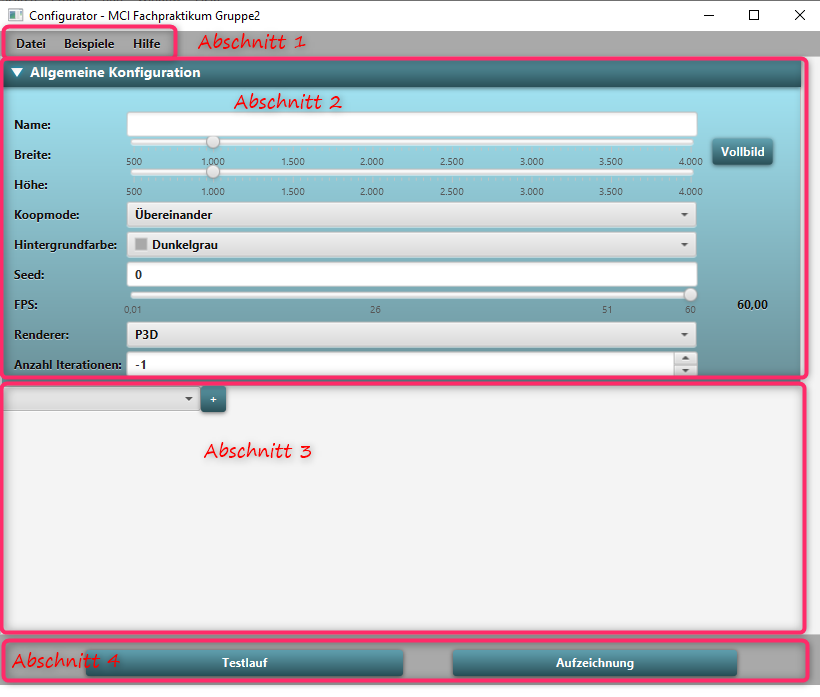
\includegraphics[width=0.5\linewidth]{"gino/all.png"}

\caption{Überblick der Benutzeroberfläche}
\end{figure}            
		
		$~$ \\In dem obigen Bild sieht man die Benutzeroberfläche beim Aufruf des Konfigurators, welche für die Interaktion mit dem User zuständig ist. Bei näherer Betrachtung lässt sich feststellen, dass die Benutzeroberfläche in vier Bereiche unterteilt werden kann.
		
		$~$ \\Der erste Bereich zeigt eine Menüleiste, welche zwei Untermenüs enthält.
		Das linke Untermenü ist das ' Datei '-Menü, welches weitere Unterpunkte beinhaltet. Hier können nun folgende Funktionen ausgeführt werden:
		
		\begin{itemize}
            % \item New: Erstellen einer neuen Konfiguration.
            \item Öffnen: Öffnen einer bereits gespeicherten Konfiguration.
			\item Öffne letzte Konfiguration: Öffnen der letzten Konfiguration.
			\item Reset: Zurücksetzen der bisher ausgwählten Konfigurationen.
            \item Speichern: Speichern der aktuellen Konfiguration.
            \item Speichern unter: Speichern der aktuellen Konfiguration unter.
            \item Schließen: Schließen des Tools.
        \end{itemize}
        
        $~$ \\In der Mitte befindet sich der Menüpunkt "Beispiele". Unter diesen Menüpunkt befinden sich vordefinierte Konfigurationen, um die erstellten Bilder zu reproduzieren. Hierfür kann ein Beispiel ausgewählt werden und anschließend werden direkt alle notwendigen Konfigurationen eingestellt. Somit erleichtert diese Funktion, die z.B. in der Ausarbeitung dargestellten Bilder zu rekonstruieren.
        Außerdem sieht man unter dem rechten Untermenü ' Hilfe ' zum einen den Unterpunkt ' Info ', welcher eine kurze Erklärung zum entwickelten Konfigurator liefert. Zum anderen befindet sich dort der Unterpunkt ' Steuerung ', wo einige Kurzbefehle beschrieben sind.
        
        $~$ \\Im zweiten Abschnitt der Benutzeroberfläche befindet sich der Bereich zu einer allgemeinen Konfiguration. Dort können allgemeine Parameter für die Ausführung des Konfigurators gesetzt werden, welche nun aufgeführt werden:
        \begin{itemize}
            \item Name: Name der Konfiguration.
            \item Breite: Breite des Bildes.
            \item Höhe: Höhe des Bildes.
            \item Koopmode: Modus der Koorperation.
            \item Hintergrundfarbe: Hintergrundfarbe des Bildes.
            \item Seed: Wert des default-Seeds.
            \item FPS: Einstellung für die Frame per second.
            \item Renderer: Einstellung für den Renderer des Bildes.
            \item Anzahl Iterationen: Bestimmt die Anzahl der Iterationen der Zeichnung
        \end{itemize}
        
        $~$ \\Nun kann der User im dritten Abschnitt der Benutzeroberfläche eine individuelle Konfiguration vornehmen. Hier kann eine beliebige Anzahl von Generatoren hinzugefügt werden. Dabei können einzelne Generatoren über das enthaltene DropDown-Menü ausgewählt werden und anschließend mithilfe des ' + ' dem Konfigurator hinzugefügt werden. Die einzelnen Generatoren können jeweils individuell parametrisiert werden, welches im weiteren Text für jeden Generator beschrieben wird.
        Zusätzlich können mithilfe der Pfeile bei jedem hinzugefügten Generator, die Reihenfolge der Generatoren verändert werden.
        
        \begin{figure}[H]
\centering
            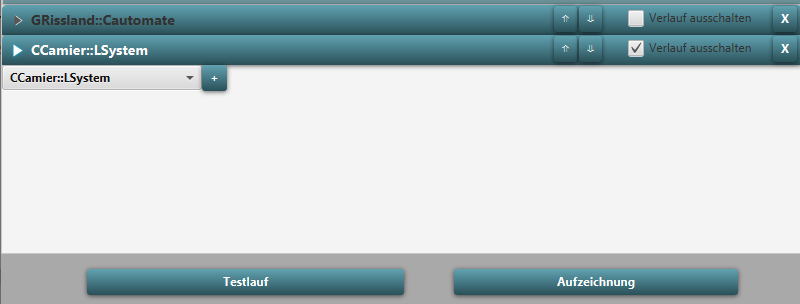
\includegraphics[width=0.5\linewidth]{"gino/config.png"}

\caption{Überblick der individuellen Konfiguration}
\end{figure}            
        
        $~$ \\Im letzten Abschnitt der Benutzeroberfläche sind zwei Button zu sehen. Dabei wird bei einem Klick auf den Button ' Testlauf ' ein Testbild gezeichnet. Der zweite Button ' Aufzeichnung ' kann dann betätigt werden, wenn z.B. eine ansprechende Konfiguration für die Zeichnung eines Bildes gefunden wurde. Nach Klick auf diesen Button wird ein weiteres Fenster geöffnet, wo eine enstprechende Aufzeichnung und ein Speicherort bestimmt werden kann. Anschließend wird dann je nach Konfiguration die Datei an dem ausgewählten Ort gespeichert.
        
        \begin{figure}[H]
\centering
            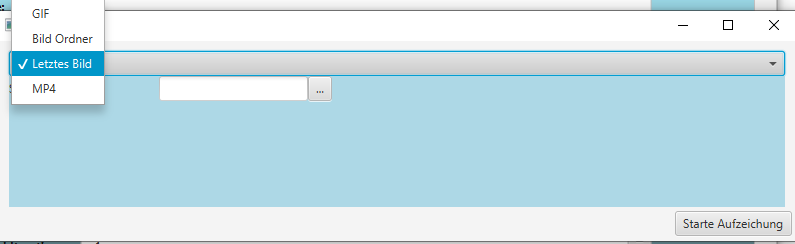
\includegraphics[width=0.5\linewidth]{"gino/Aufzeichnung.png"}

\caption{Überblick Aufzeichnungsmenü}
\end{figure}          


\end{document}